%% ===========================================================================
%% An Empirical Comparison of Process- and Thread-Based Parallelization
%% Strategies for Ant Colony Optimization in Grid Path Planning
%%
%% IEEE conference format. Compile on Overleaf (easiest) or locally:
%%   pdflatex main && bibtex main && pdflatex main && pdflatex main
%%
%% Figures are read from ../results/figures/ (run bench/plots.py first).
%% Markers like [[FILL: ...]] flag things you must complete before submission.
%% ===========================================================================
\documentclass[conference]{IEEEtran}
\IEEEoverridecommandlockouts
\usepackage{cite}
\usepackage{amsmath,amssymb}
\usepackage{graphicx}
\usepackage{booktabs}
\usepackage{url}
\graphicspath{{../results/figures/}}

\begin{document}

\title{An Empirical Comparison of Process- and Thread-Based\\
Parallelization Strategies for Ant Colony Optimization\\
in Grid-Based Path Planning}

\author{\IEEEauthorblockN{Gottipati Harshith Sai}
\IEEEauthorblockA{\textit{[[FILL: Department]]} \\
\textit{[[FILL: University]]}\\
[[FILL: City, Country]] \\
gharshithsai03@gmail.com}}

\maketitle

\begin{abstract}
Ant Colony Optimization (ACO) is a population-based metaheuristic whose
per-iteration ant exploration is embarrassingly parallel, making it a natural
candidate for multi-core acceleration. We present a controlled empirical study
comparing two parallelization strategies for ACO applied to obstacle-laden grid
path planning: process-based parallelism using Python's \texttt{multiprocessing}
and thread-based shared-memory parallelism using C with OpenMP. Both implement
the identical algorithm; we hold the workload fixed and vary the worker count
from 1 to 16 on an 8-core (16-thread) AMD Ryzen 7 7840HS, measuring speedup,
parallel efficiency, and solution quality. The C/OpenMP implementation reaches a
speedup of $5.7\times$ while the Python implementation saturates at $4.6\times$,
limited by per-iteration data serialization; an Amdahl's-law fit estimates a
serial fraction of $10.8\%$. We also find that, per iteration, the C/OpenMP
solver is roughly $94\times$ faster than the Python multiprocessing one, and that
process-based parallelism with a single worker is actually \emph{slower} than a
pure-serial baseline. We further characterize solution quality as a function of
obstacle density. Our results quantify the practical cost of process-based
parallelism for fine-grained metaheuristics and provide a reproducible benchmark.
\end{abstract}

\begin{IEEEkeywords}
ant colony optimization, parallel computing, OpenMP, multiprocessing,
path planning, Amdahl's law, strong scaling
\end{IEEEkeywords}

% ===========================================================================
\section{Introduction}
Grid-based path planning---finding a short, collision-free route for an agent
from a start cell to a goal cell---is a core problem in robotics and games.
Ant Colony Optimization (ACO)~\cite{dorigo1996ant,dorigo2004aco} solves it by
having many simple agents (``ants'') construct candidate paths that are
probabilistically biased by accumulated \emph{pheromone} and a greedy
\emph{heuristic}. Because each ant builds its path independently within an
iteration, ACO exposes abundant parallelism.

How that parallelism is realized, however, has a large practical effect. This
paper asks a focused question: \emph{for fine-grained ACO path planning, how do
process-based and thread-based parallelization strategies compare in speedup,
efficiency, and solution quality?}

\textbf{Contributions.} (1)~A reproducible benchmark harness that runs an
identical ACO algorithm under two parallel back-ends---Python
\texttt{multiprocessing} and C/OpenMP. (2)~A strong-scaling analysis with an
Amdahl's-law characterization of the serial bottleneck. (3)~A quantification of
the serialization overhead that limits process-based parallelism for this
workload. (4)~A study of solution quality versus obstacle density.

% ===========================================================================
\section{Related Work}
\label{sec:related}
\textbf{ACO and its variants.} ACO was introduced as the Ant
System~\cite{dorigo1996ant} and strengthened by the Ant Colony
System~\cite{dorigo1997acs} and the MAX--MIN Ant System~\cite{stutzle2000maxmin},
which bounds pheromone values to avoid premature convergence; comprehensive
treatments appear in~\cite{dorigo2004aco,dorigo2006aco}. We adopt a standard
Ant-System-style pheromone update and do not propose an algorithmic variant; our
focus is the parallel execution model.

\textbf{ACO for path planning.} ACO is widely used for mobile-robot and
grid-based path planning. Ali et al.~\cite{ali2020pathplanning} combine an
improved ACO with a Markov decision process to smooth trajectories in grid
environments, while island- and pheromone-initialization schemes target faster
convergence and deadlock avoidance~\cite{li2024islands}. These works improve
\emph{solution quality} on a sequential solver, whereas we study how the choice of
parallel execution affects \emph{performance}.

\textbf{Parallel and GPU ACO.} Because ant path construction is independent within
an iteration, ACO parallelizes naturally; Pedemonte et al. survey the design
space~\cite{pedemonte2011survey}. Early CPU strategies include parallel
independent runs and master--worker schemes~\cite{stutzle1998parallel,randall2002parallel},
and GPU implementations report large speedups via fine-grained data
parallelism~\cite{delevacq2013gpu,cecilia2013enhancing}. Closest to our
application, Si and Bao~\cite{si2024parallel} propose a parallel ACO for robot path
planning. Unlike these efforts---which propose new parallel \emph{algorithms} or
target GPUs---we hold a single algorithm fixed and empirically contrast two CPU
execution models, process-based (Python \texttt{multiprocessing}) versus
thread-based (C/OpenMP), on identical instances, isolating the data-movement cost
intrinsic to process-based parallelism.

\textbf{Performance modeling.} Parallel scaling is classically bounded by
Amdahl's law~\cite{amdahl1967}, with the scaled-workload view from
Gustafson~\cite{gustafson1988}; we use OpenMP~\cite{dagum1998openmp} as the
shared-memory model and fit Amdahl's law to our measured speedup.

% ===========================================================================
\section{Background: ACO for Grid Path Planning}
The environment is an $N\times N$ grid; each cell is free or an obstacle, with
8-connected moves. An ant at cell $i$ chooses the next free, unvisited cell $j$
with probability
\begin{equation}
p_{ij} = \frac{\tau_{ij}^{\alpha}\,\eta_{ij}^{\beta}}
              {\sum_{k \in \mathcal{N}_i} \tau_{ik}^{\alpha}\,\eta_{ik}^{\beta}},
\end{equation}
where $\tau_{ij}$ is the pheromone on cell $j$, $\eta_{ij}=1/d(j,\text{goal})$ is
the heuristic (inverse distance to goal), and $\alpha,\beta$ weight their
influence. After every ant completes an iteration, pheromone evaporates and
successful ants deposit pheromone:
\begin{equation}
\tau_{ij} \leftarrow (1-\rho)\,\tau_{ij} + \sum_{a}\Delta\tau_{ij}^{a},
\qquad \Delta\tau_{ij}^{a} = Q/L_a,
\end{equation}
where $\rho$ is the evaporation rate, $L_a$ the length of ant $a$'s path, and $Q$
a constant. Path construction (the dominant cost) is parallel across ants; the
evaporation/deposit update is serial, defining the Amdahl bottleneck.

% ===========================================================================
\section{Parallelization Strategies}
Both implementations parallelize the same loop---ant path construction within an
iteration---and keep the pheromone update serial.

\subsection{Thread-based (C / OpenMP)}
Ants share the read-only pheromone matrix; the ant loop is annotated with
\texttt{\#pragma omp parallel for schedule(dynamic)}. No per-ant data copying is
required because memory is shared.

\subsection{Process-based (Python \texttt{multiprocessing})}
Each ant is dispatched to a worker process via \texttt{Pool.map}. Because
processes do not share memory, the pheromone matrix is serialized (pickled) and
sent to workers \emph{every iteration}---the key overhead we quantify.

% ===========================================================================
\section{Experimental Setup}
\label{sec:setup}
Experiments were run on an AMD Ryzen 7 7840HS (8 physical / 16 logical cores),
16\,GB RAM, Windows 11 (build 26200), Python 3.11.9 (NumPy 1.24.3), and GCC 13.2.0
with \texttt{-O2 -fopenmp}. The exact environment is recorded in
\texttt{results/platform.json}.

\textbf{Workload (strong scaling).} $N=48$, obstacle density $=0.20$, $200$ ants,
$100$ iterations, $\alpha{=}1.0$, $\beta{=}2.5$, $\rho{=}0.1$. Worker count is
swept over $\{1,2,4,8,12,16\}$. Each configuration is repeated $5$ times after a
discarded warm-up run; we report the mean and a 95\% confidence interval. Ant
random seeds are fixed per iteration, so solution quality is identical across
worker counts and we measure \emph{pure} speedup.
We define speedup $S(p)=T(1)/T(p)$ and efficiency $E(p)=S(p)/p$, where $T(p)$ is
the mean per-iteration time at $p$ workers.

\textbf{Quality experiment.} For the density study (\S\ref{sec:results}) we
generate, for each density, a single obstacle layout at the \emph{exact} target
density that is verified feasible by breadth-first search, and solve that same
shared instance with both back-ends. This removes any layout or
feasibility-handling asymmetry between the two implementations.

% ===========================================================================
\section{Results}
\label{sec:results}
\subsection{Strong scaling}
Fig.~\ref{fig:runtime} shows per-iteration time and Fig.~\ref{fig:speedup} the
resulting speedup. The C/OpenMP solver scales to a peak of $5.7\times$ at $12$
threads and then plateaus (slightly regressing to $5.5\times$ at $16$), consistent
with the machine having only $8$ physical cores---beyond which simultaneous
multithreading yields little. Python multiprocessing scales more gradually to
$4.6\times$ at $16$ workers. The Amdahl fit to the C/OpenMP data estimates a
serial fraction of $10.8\%$, consistent with the serial pheromone
evaporation/deposit update. Fig.~\ref{fig:efficiency} shows efficiency decaying
from $1.0$ as workers increase, falling faster for the process-based back-end.

\begin{figure}[t]\centering
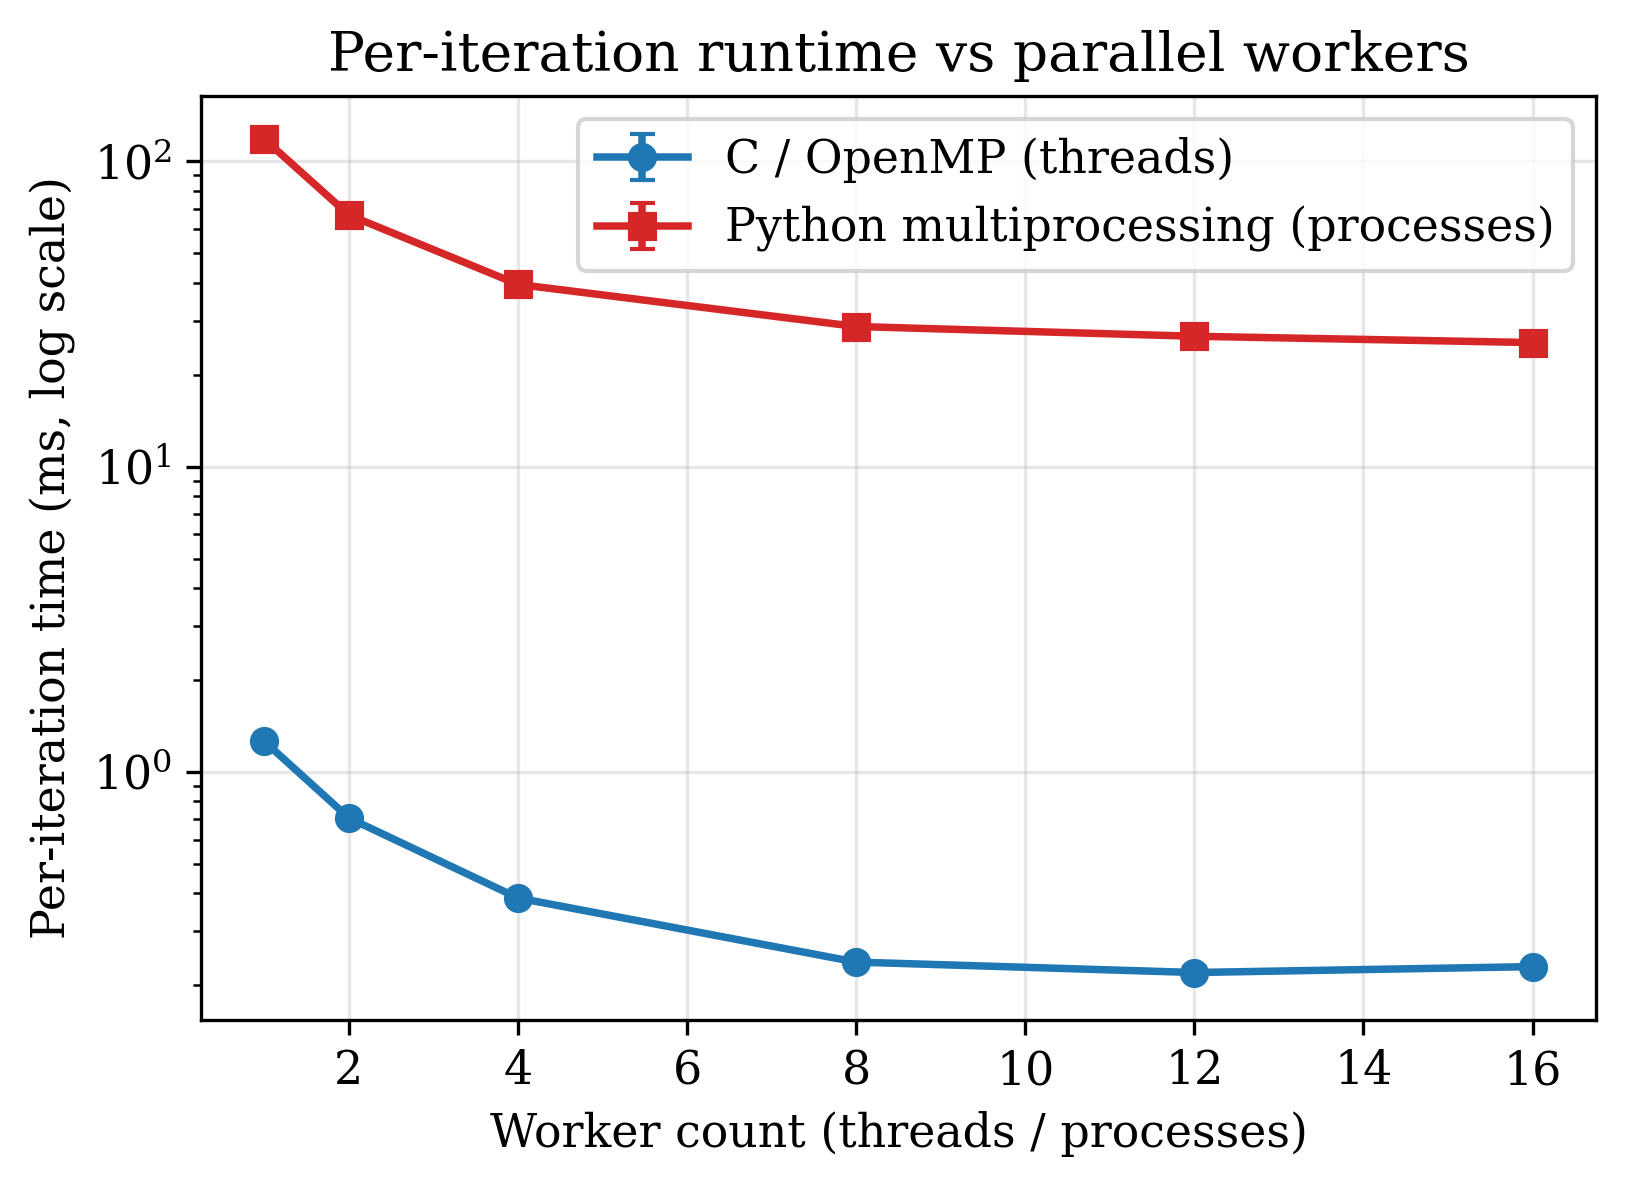
\includegraphics[width=\columnwidth]{fig_runtime.png}
\caption{Per-iteration runtime vs worker count (log scale). C/OpenMP is roughly
two orders of magnitude faster per iteration than Python multiprocessing.}
\label{fig:runtime}\end{figure}

\begin{figure}[t]\centering
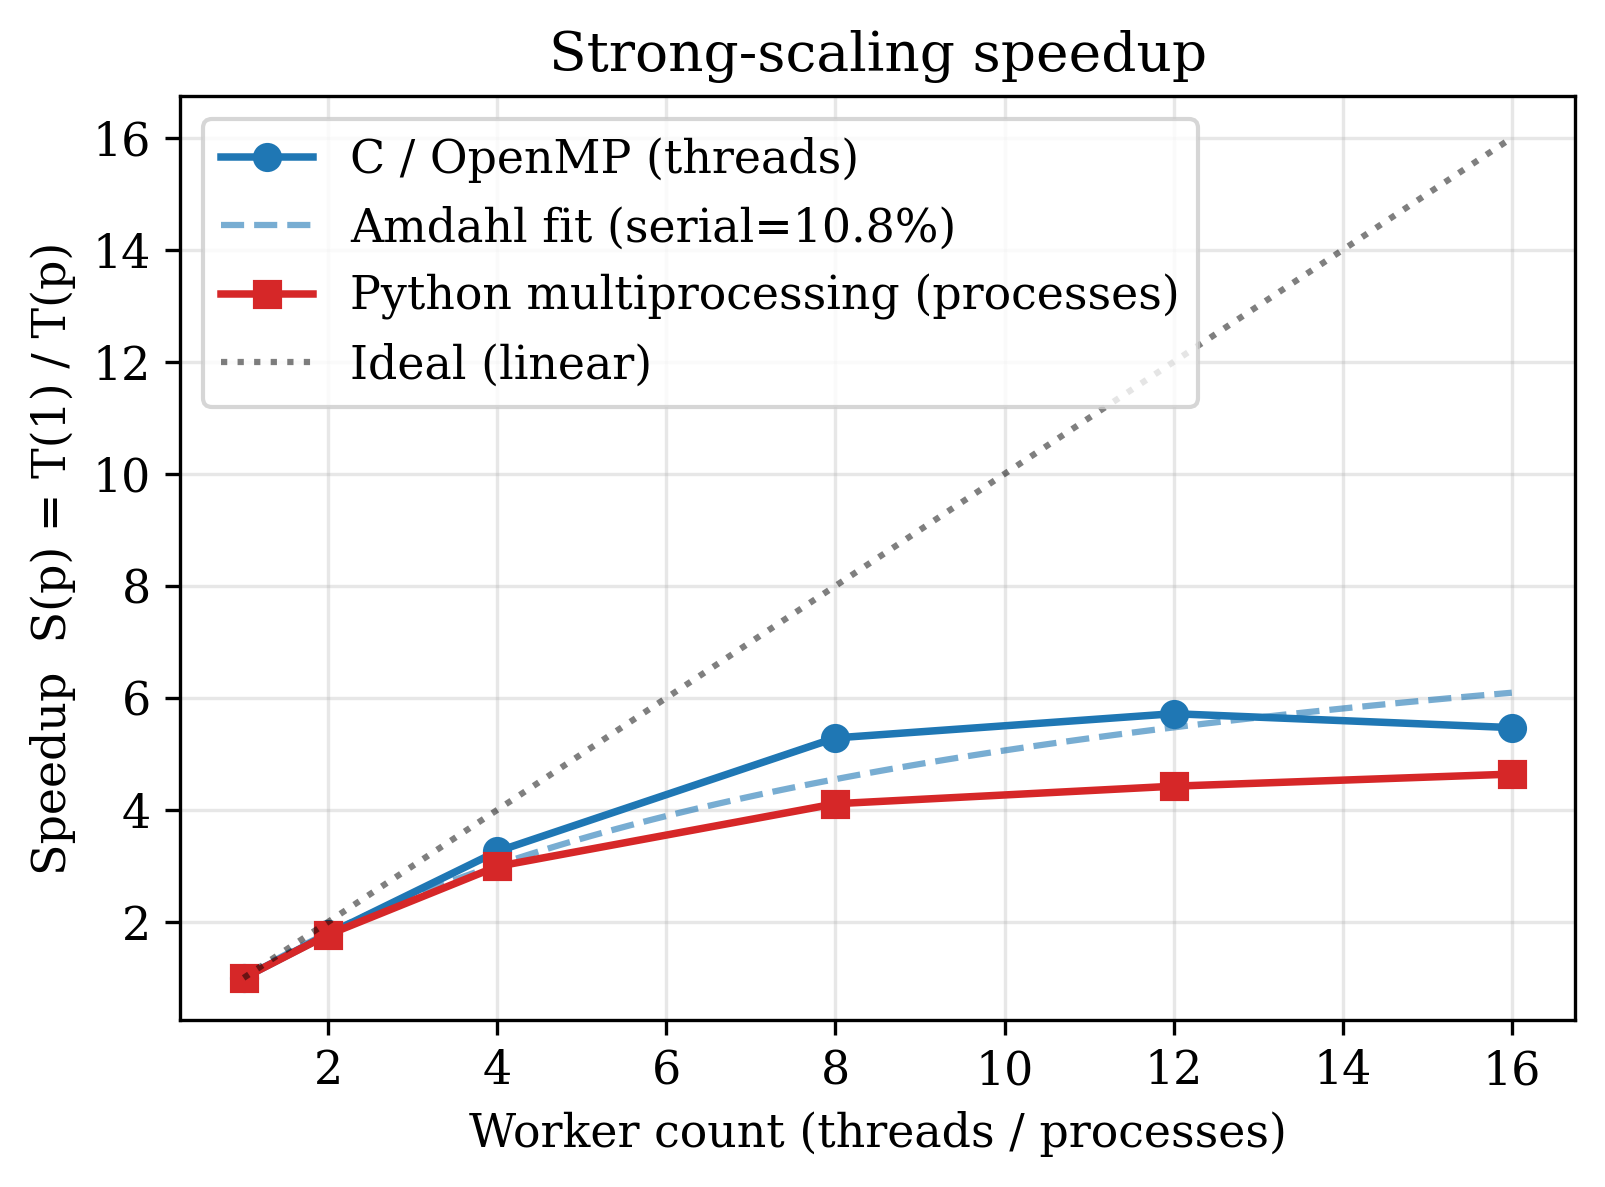
\includegraphics[width=\columnwidth]{fig_speedup.png}
\caption{Strong-scaling speedup with Amdahl's-law fit for C/OpenMP and the ideal
linear reference.}
\label{fig:speedup}\end{figure}

\begin{figure}[t]\centering
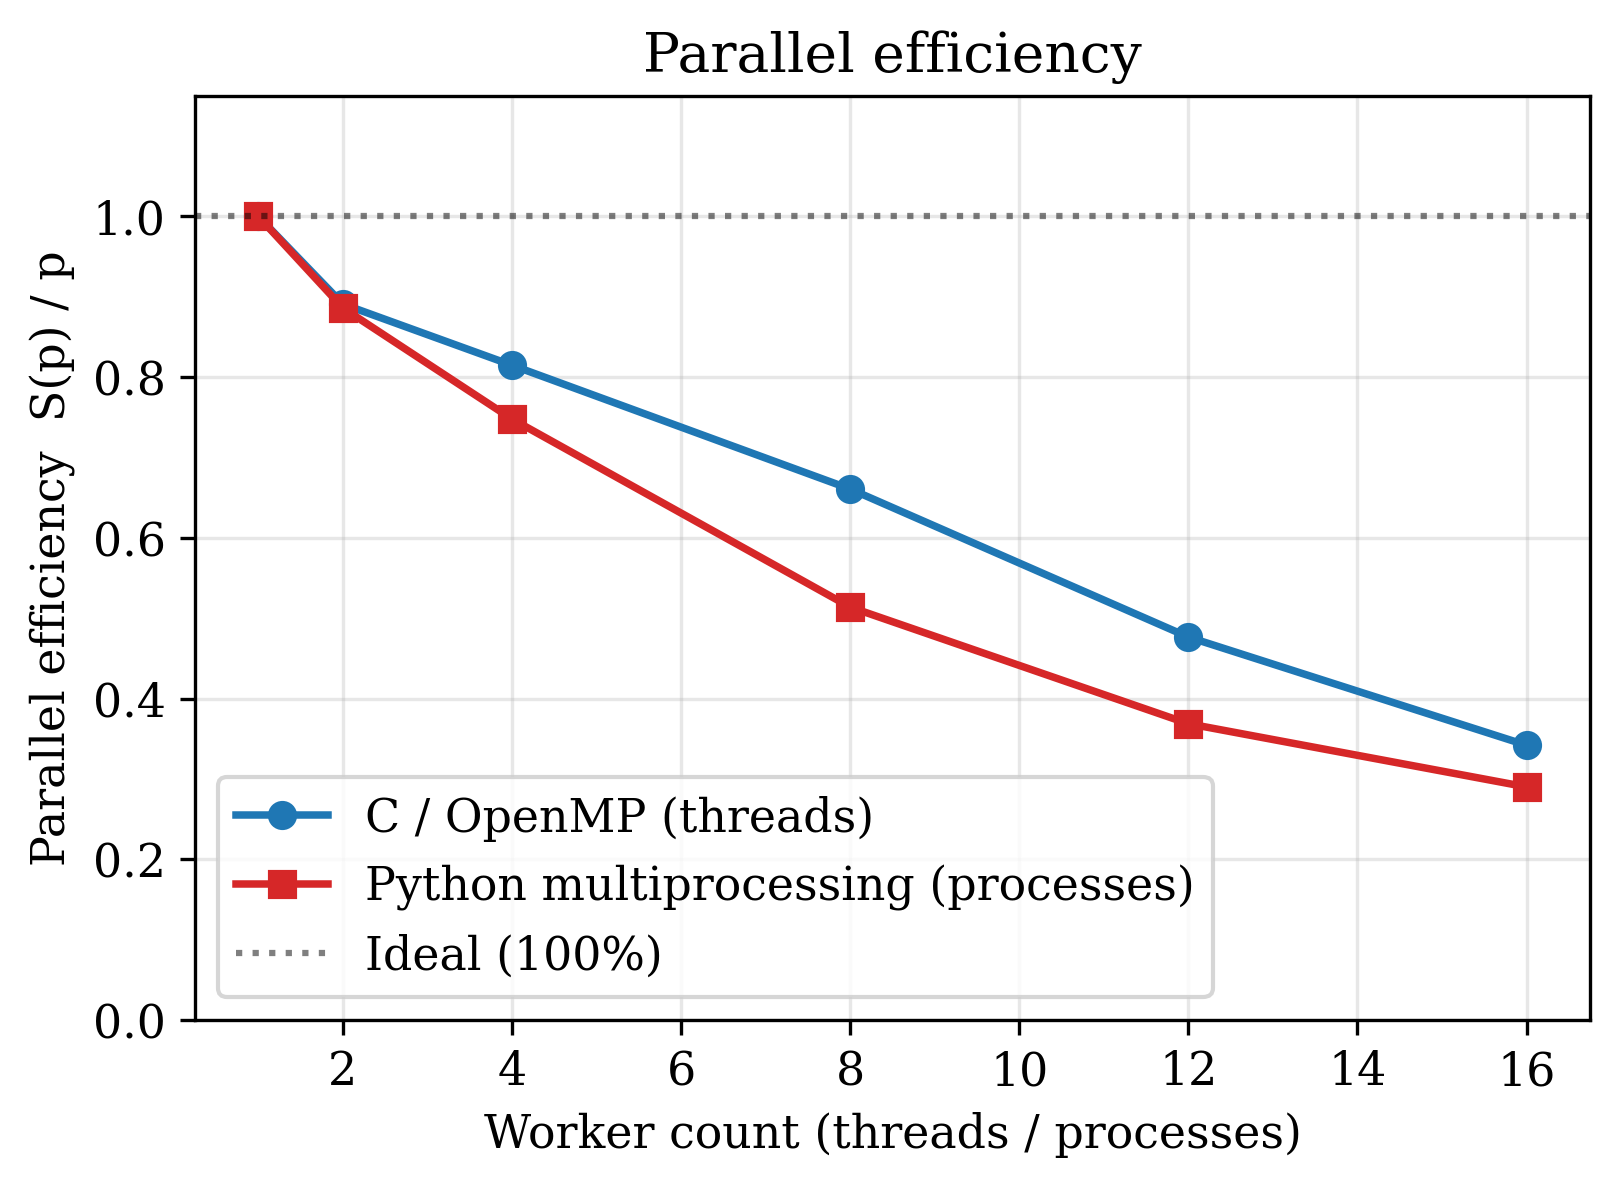
\includegraphics[width=\columnwidth]{fig_efficiency.png}
\caption{Parallel efficiency $S(p)/p$.}
\label{fig:efficiency}\end{figure}

\subsection{Serialization overhead}
Notably, Python \texttt{multiprocessing} with a single worker is \emph{slower}
than the pure-serial Python baseline ($118.3$\,ms vs $109.8$\,ms mean
per-iteration time), because inter-process data transfer---pickling the pheromone
matrix to the worker each iteration---is incurred without any parallel benefit.
Per iteration at one worker, the C/OpenMP solver ($1.26$\,ms) is about
$94\times$ faster than the Python multiprocessing one ($118.3$\,ms). Together these
isolate the cost of process-based parallelism for fine-grained tasks.

\subsection{Solution quality vs obstacle density}
For this experiment both back-ends solve the \emph{identical} grid at each
density: we generate one obstacle layout at the exact target density, verify with
breadth-first search that a start--goal path exists, and feed the same instance to
both implementations (\S\ref{sec:setup}). Fig.~\ref{fig:quality} reports best path
length as obstacle density increases. Both implementations achieve a $100\%$
success rate across all tested densities ($0.05$--$0.40$) and produce paths of
comparable length---within roughly $10$ units of one another at every density,
with overlapping 95\% confidence intervals---confirming that the two
implementations are algorithmically equivalent and that the parallelization
strategy does not affect solution quality. Path length tends to decrease slightly
at higher densities for these instances, because denser obstacle fields prune long
detours and constrain ants toward more direct routes.

\begin{figure}[t]\centering
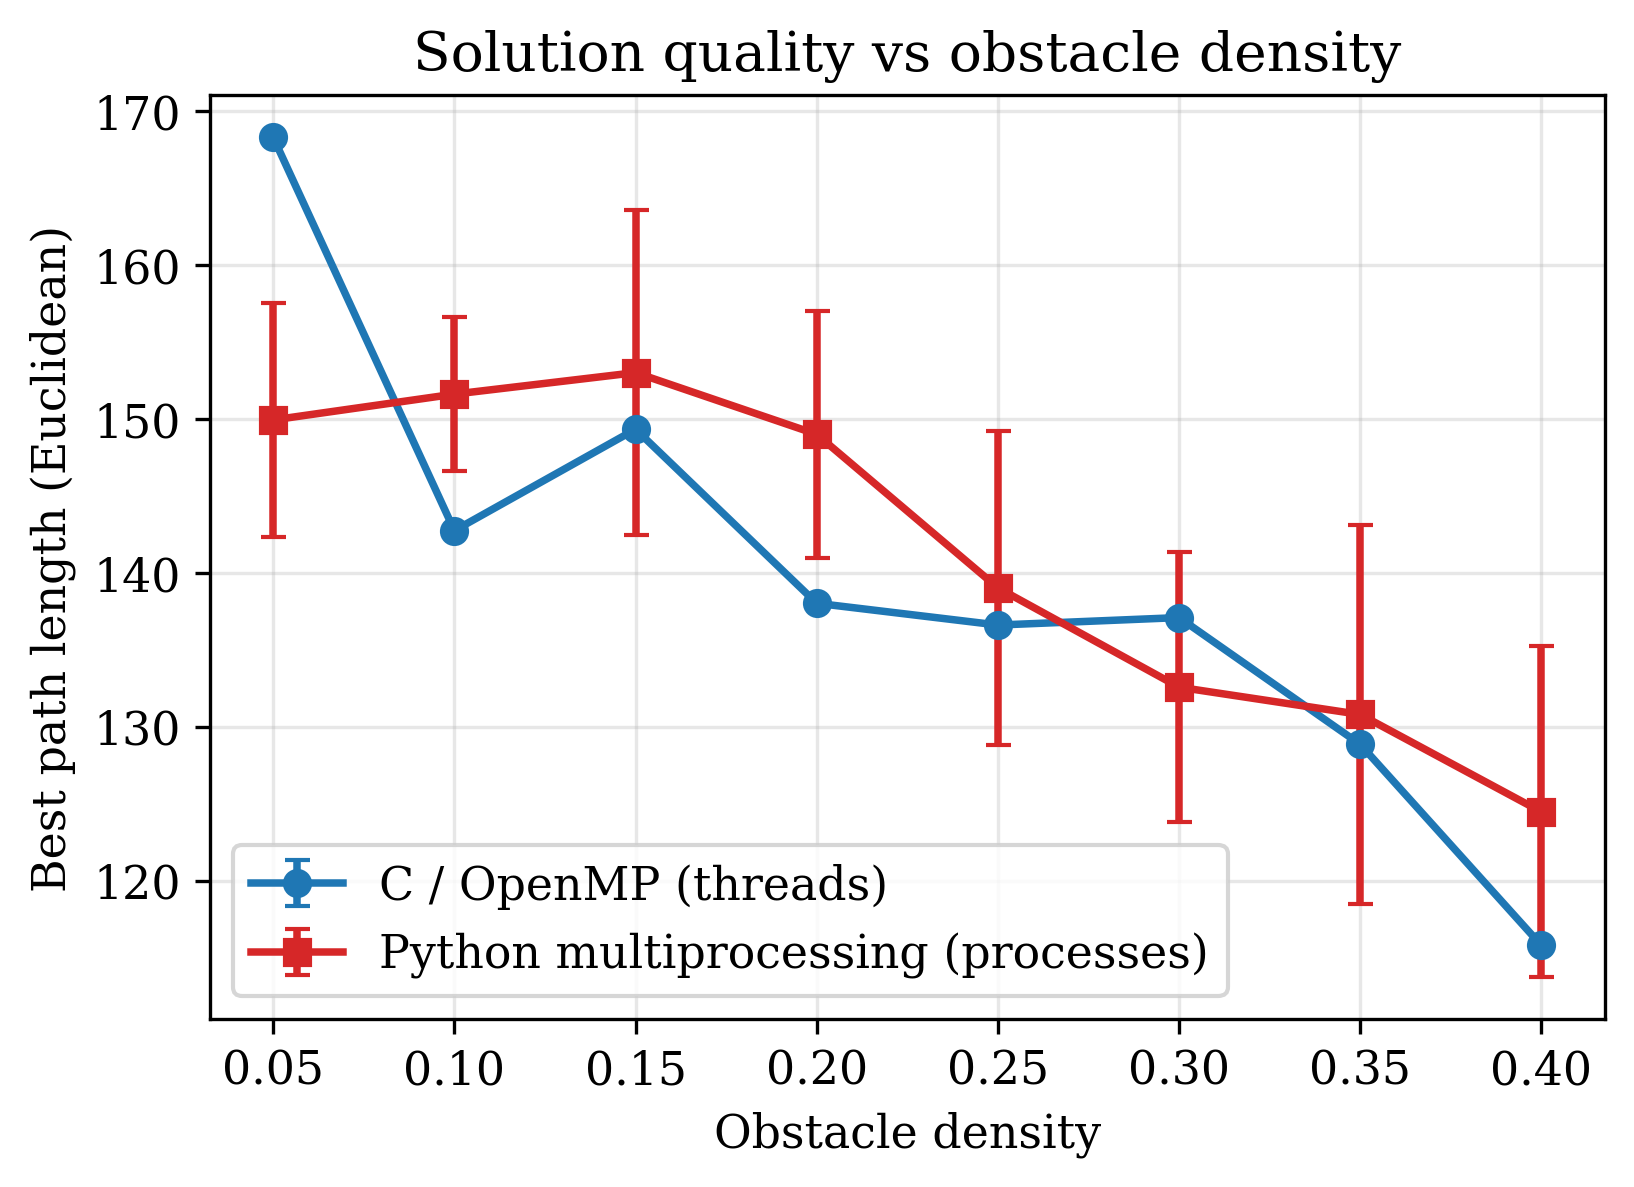
\includegraphics[width=\columnwidth]{fig_quality_density.png}
\caption{Best path length vs obstacle density (mean $\pm$ 95\% CI).}
\label{fig:quality}\end{figure}

% ===========================================================================
\section{Discussion and Limitations}
Several limitations bound our claims. The C solver caps the grid at $N\le 50$
(static allocation); larger maps would require dynamic allocation, and the scaling
study uses a single workload size. The quality study uses one feasible instance
per density; a larger battery of instances and seeds per density would tighten the
quality estimates. Finally, results are single-machine and single-architecture;
distributed-memory (e.g.\ MPI) scaling and a GPU implementation are left to future
work.

% ===========================================================================
\section{Conclusion}
We presented a reproducible, controlled comparison of process- and thread-based
parallel ACO for grid path planning. On an 8-core machine, shared-memory C/OpenMP
reached a $5.7\times$ speedup (Amdahl serial fraction $10.8\%$) and was about
$94\times$ faster per iteration than Python multiprocessing, which saturated at
$4.6\times$ and---owing to per-iteration data serialization---was even slower than
serial Python at a single worker. For fine-grained metaheuristics like ACO, the
execution model matters as much as the algorithm: shared-memory threading avoids
the data-movement tax that limits process-based parallelism. Future work includes
distributed-memory (MPI) and GPU back-ends, larger maps, and a broader battery of
instances per density.

\bibliographystyle{IEEEtran}
\bibliography{refs}

\end{document}
